\chapter*{Supplementary Information}

\section*{Data sets}

\begin{table}[h]
  \begin{threeparttable}
    \caption{Public Data sets Analyzed}
    \begin{tabular}{@{}llll@{}}
      \toprule
      Data set & Figure &  Accession & Reference \\
      \midrule % column names

      UCSC Genes &  &  &~\bibentry{karolchik2013} \\
      Lung Fibroblast Hi-C, \gls{hESC} Hi-C & GSE43070 &  &~\bibentry{jin2013} \\
      COSMIC Lung Cancer Mutations & &  &~\bibentry{forbes2009} \\
      H1 \gls{hESC} Gene Signatures & GSE54186 & &~\bibentry{kim2014} \\
      IMR90 Gene Signatures & GSE2672 & &~\bibentry{kim2005} \\
      \bottomrule
    \end{tabular}
    \begin{tablenotes}
      All of these data sets were obtained as of December 2014.
    \end{tablenotes}
  \end{threeparttable}
\end{table}


\section*{Gene Expression Histograms}

\begin{figure}[ht]
  \centering
  \subfigure[IMR90 Expression Data]{%
    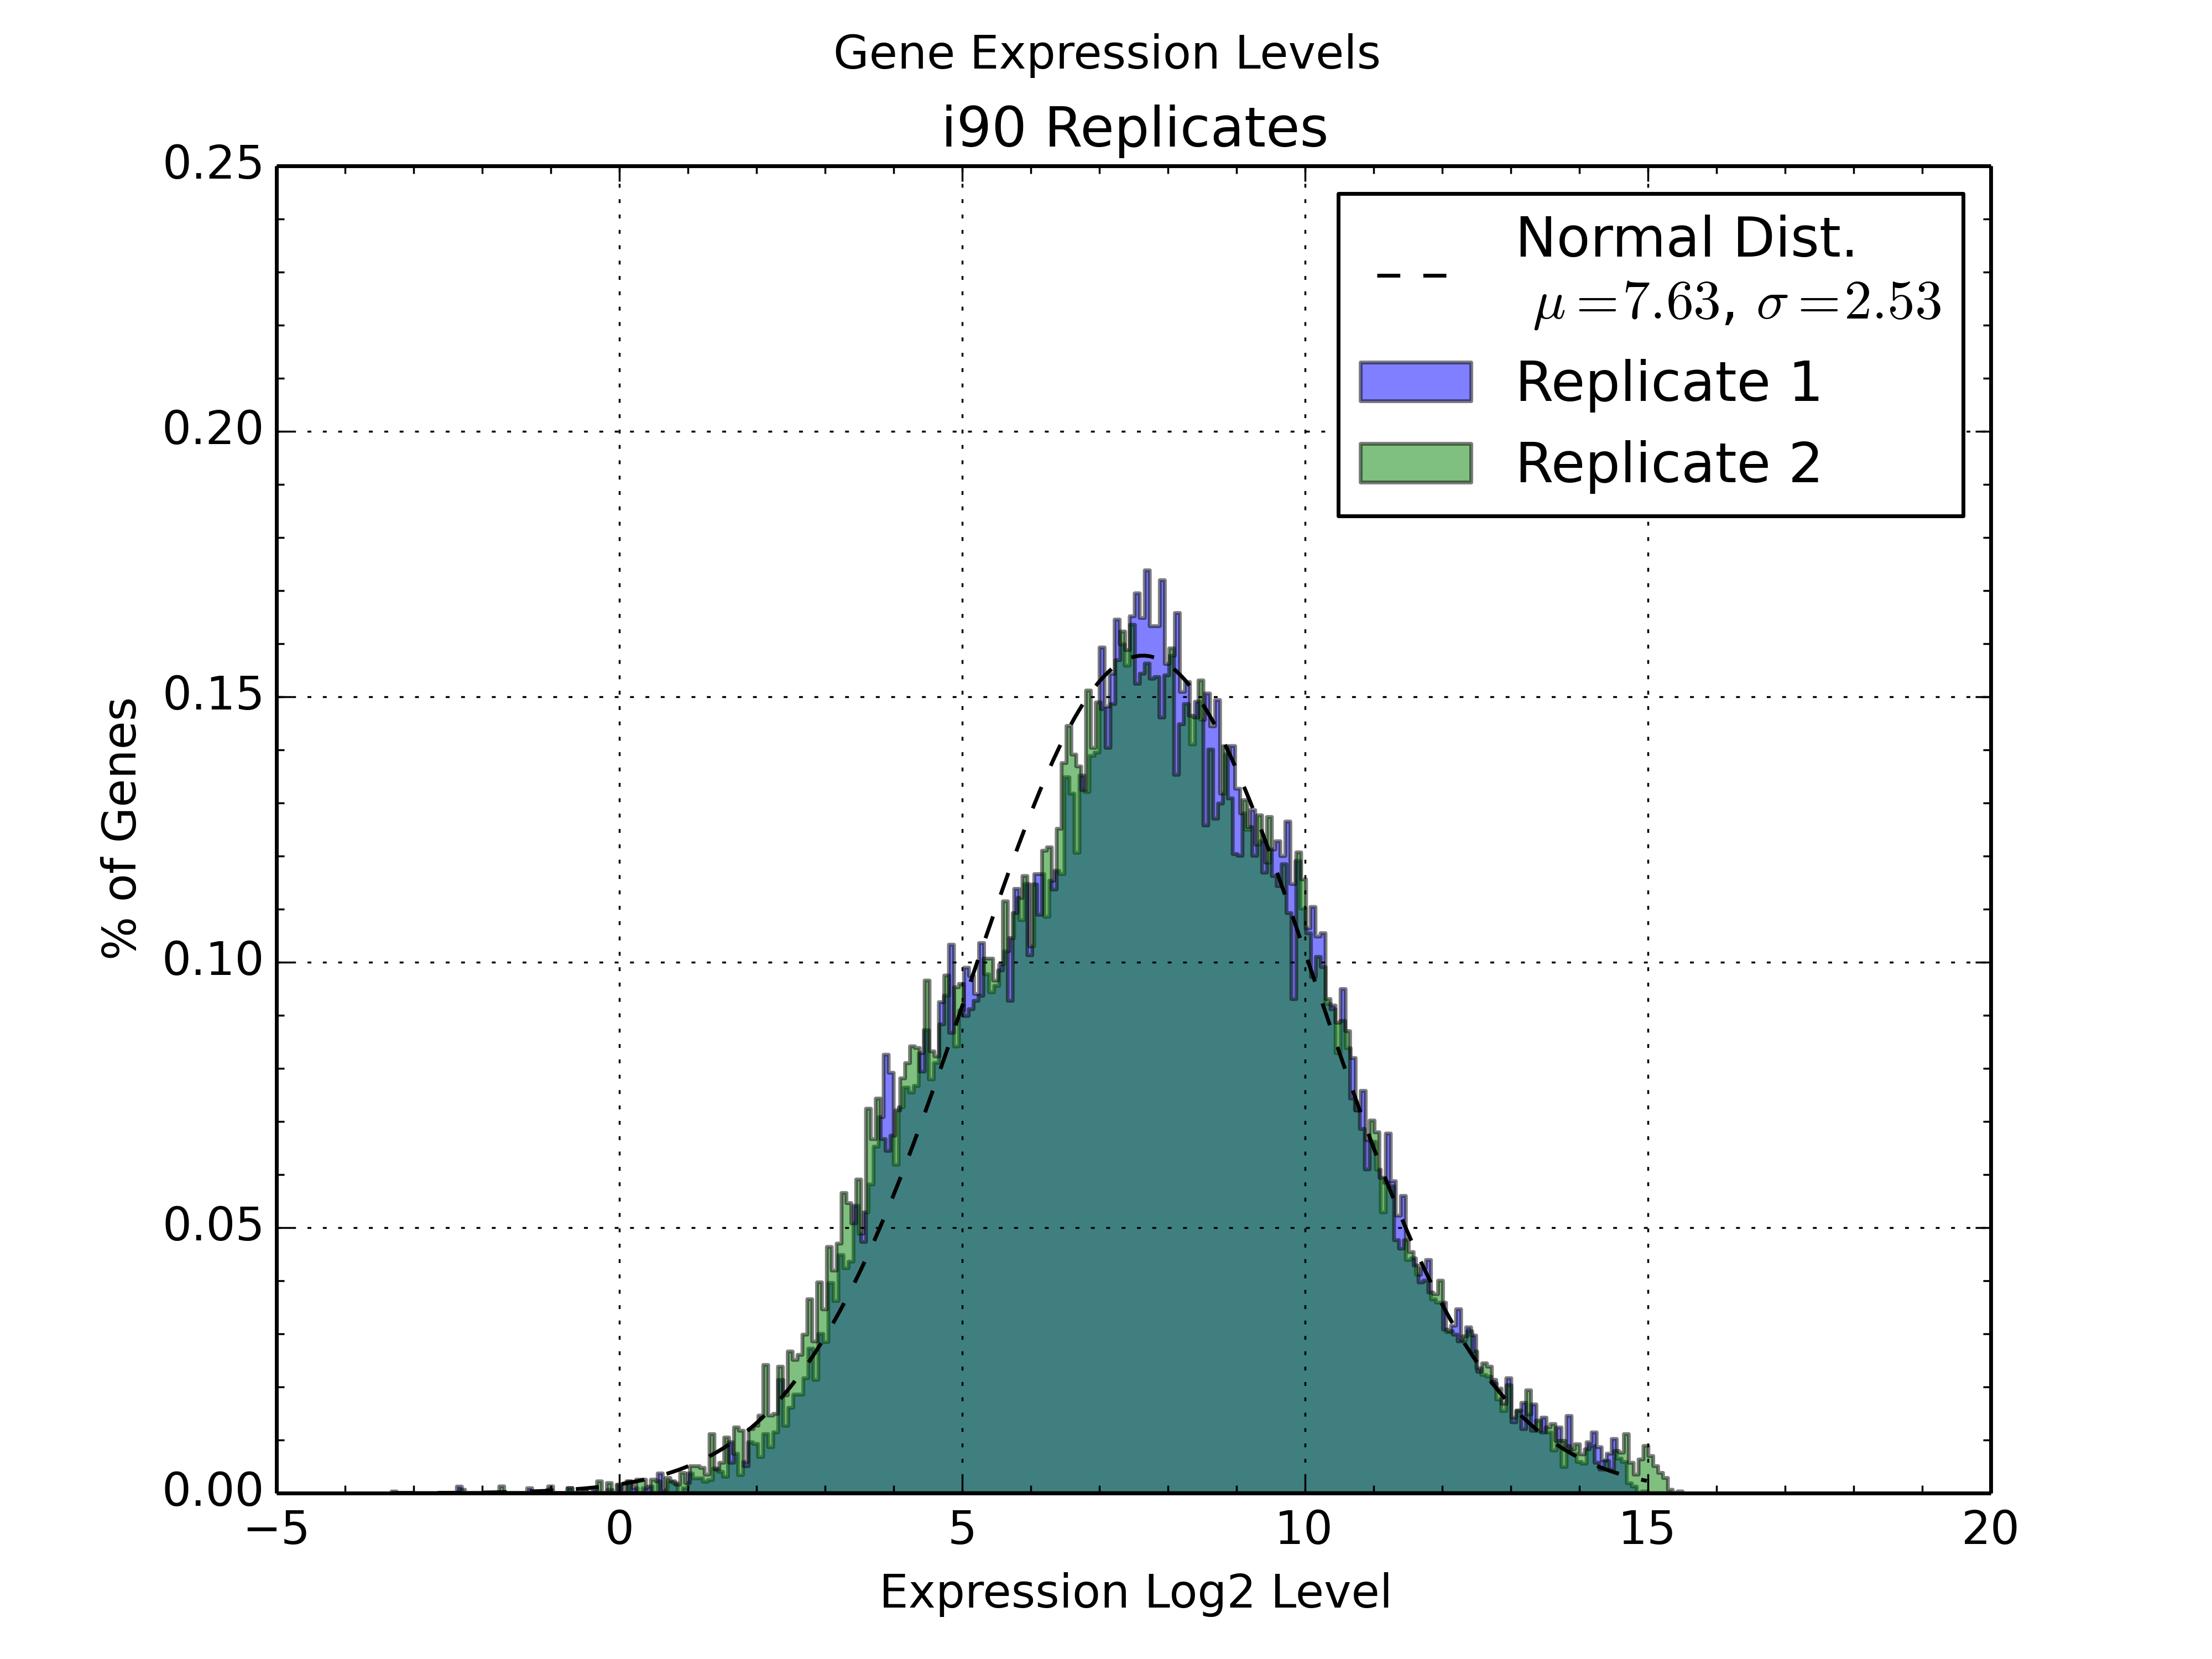
\includegraphics{./fig/supplementary/i90-expression-levels.png}\label{fig:subfigure1}
  }
  \quad
  \subfigure[H1 hESC Expression Data]{%
    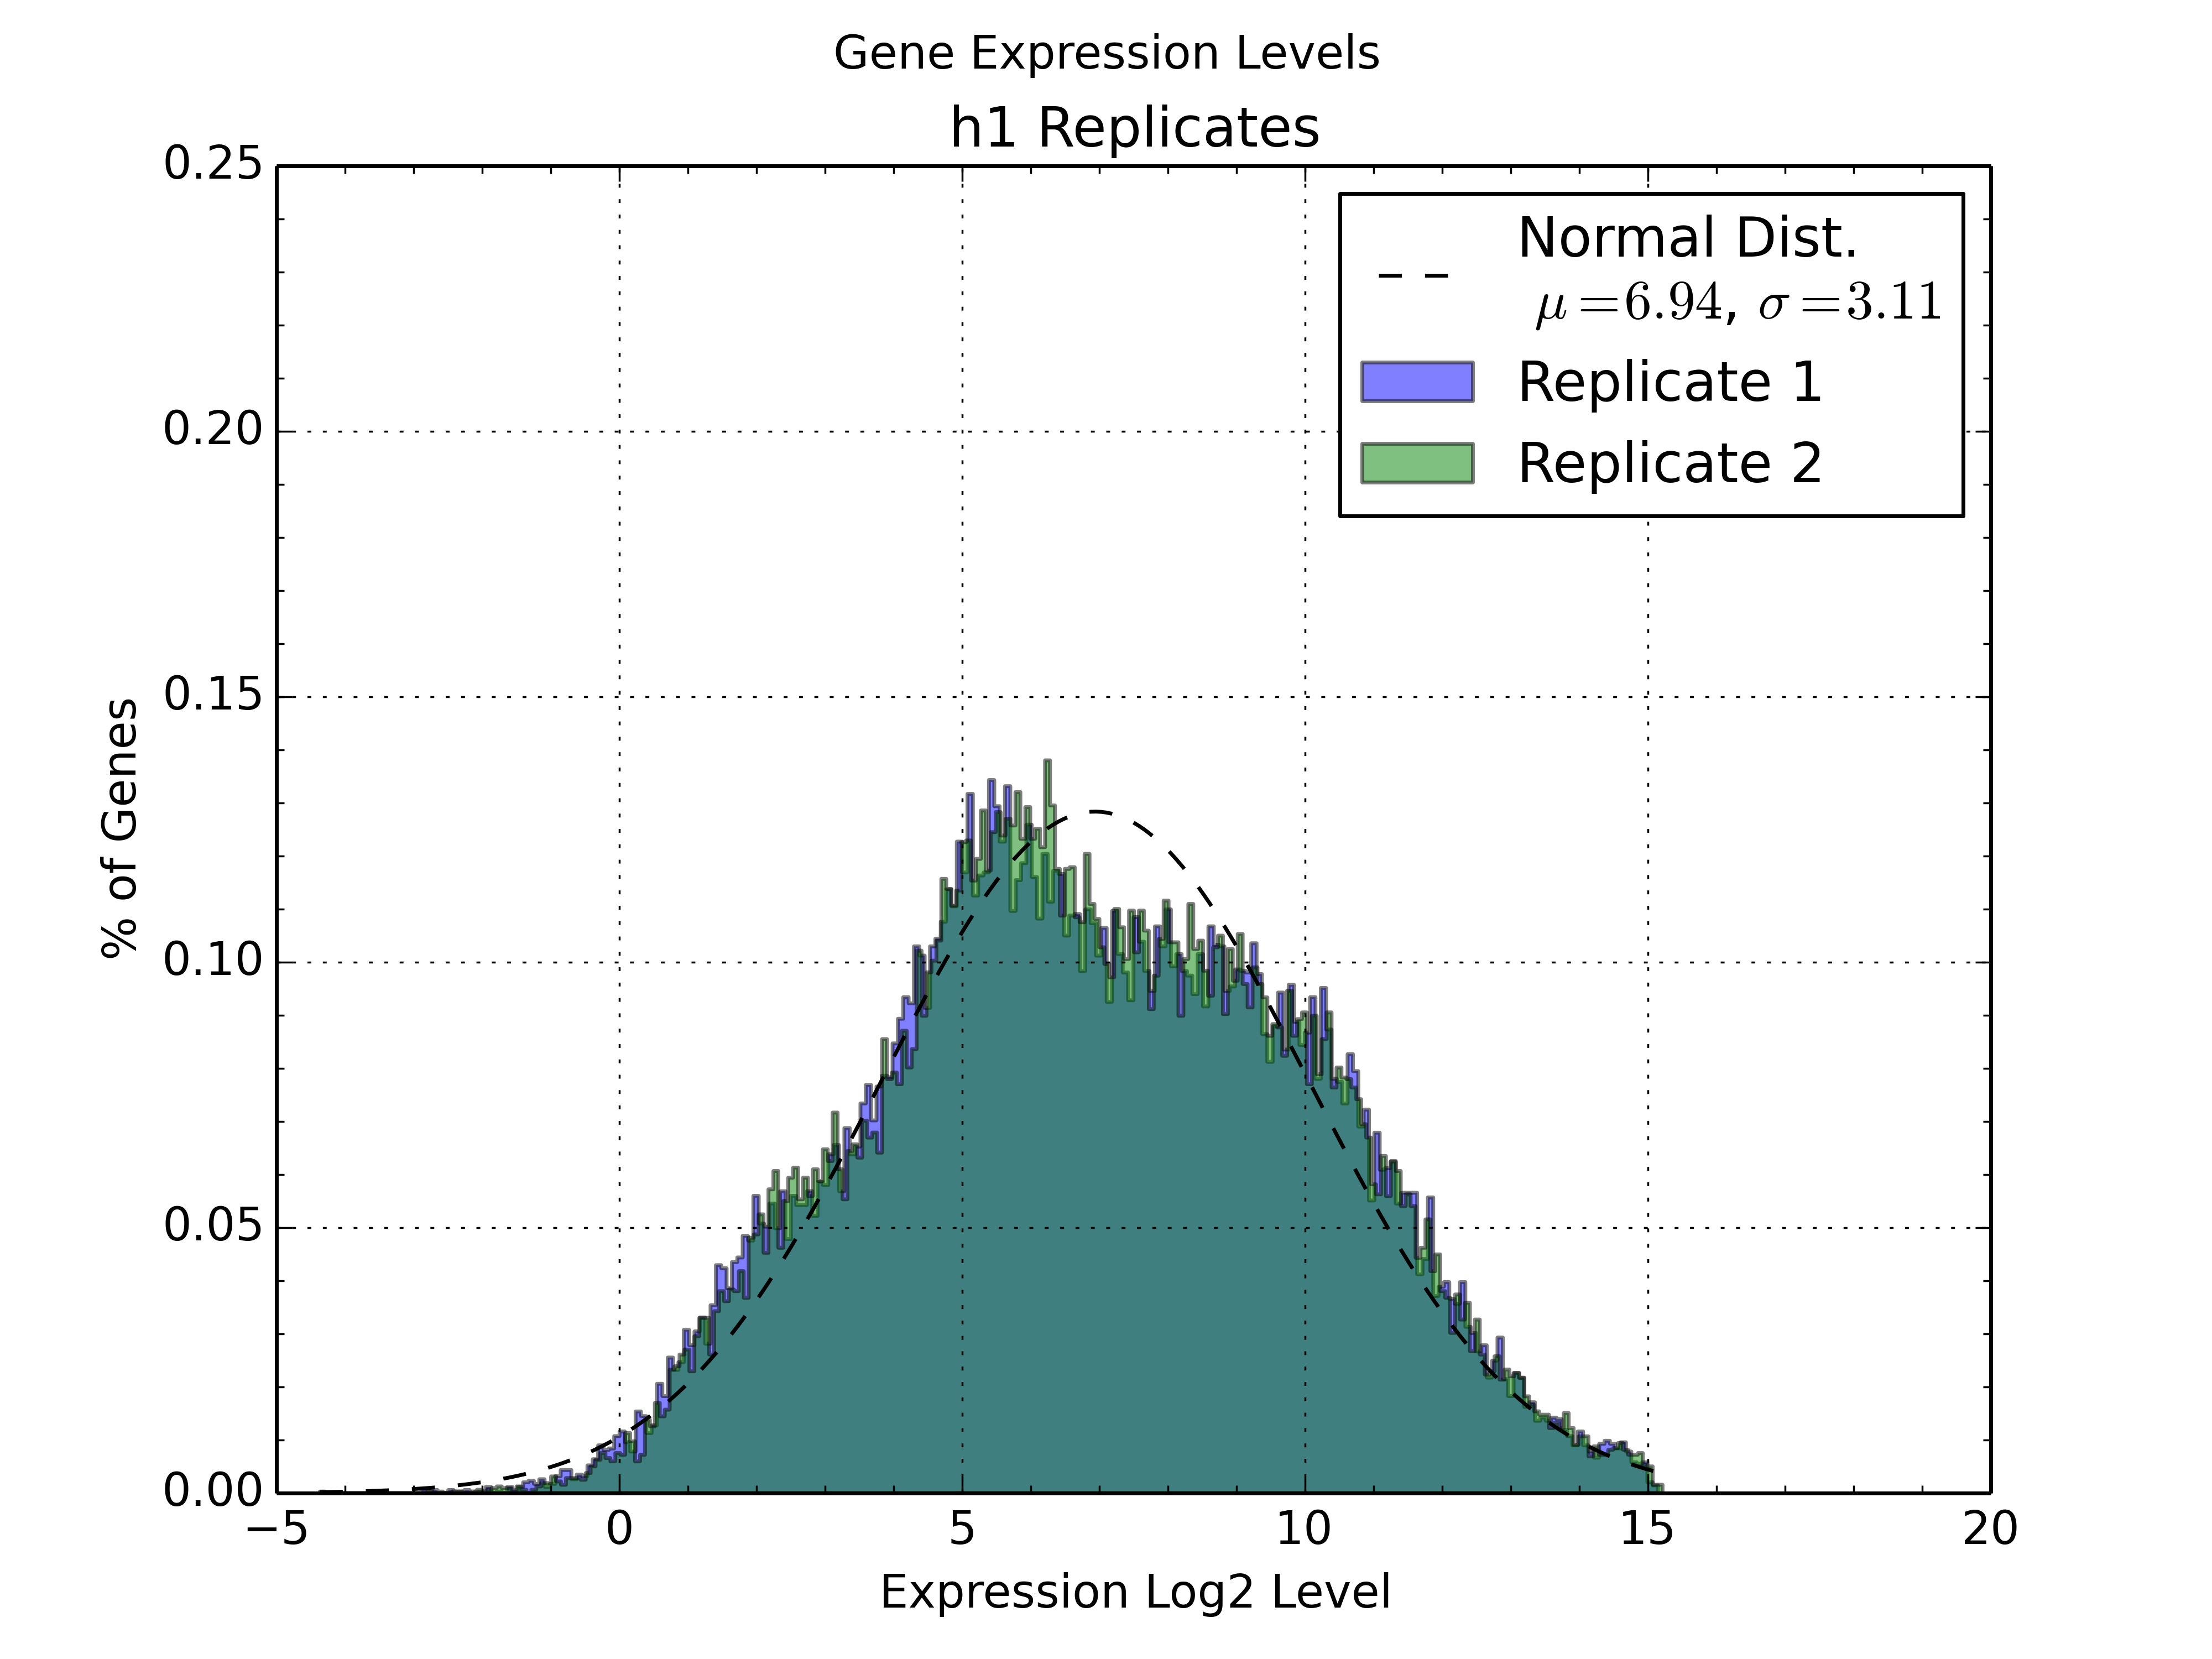
\includegraphics{./fig/supplementary/h1-expression-levels.png}\label{fig:subfigure2}
  }

  \subfigure[Expression Changes]{%
    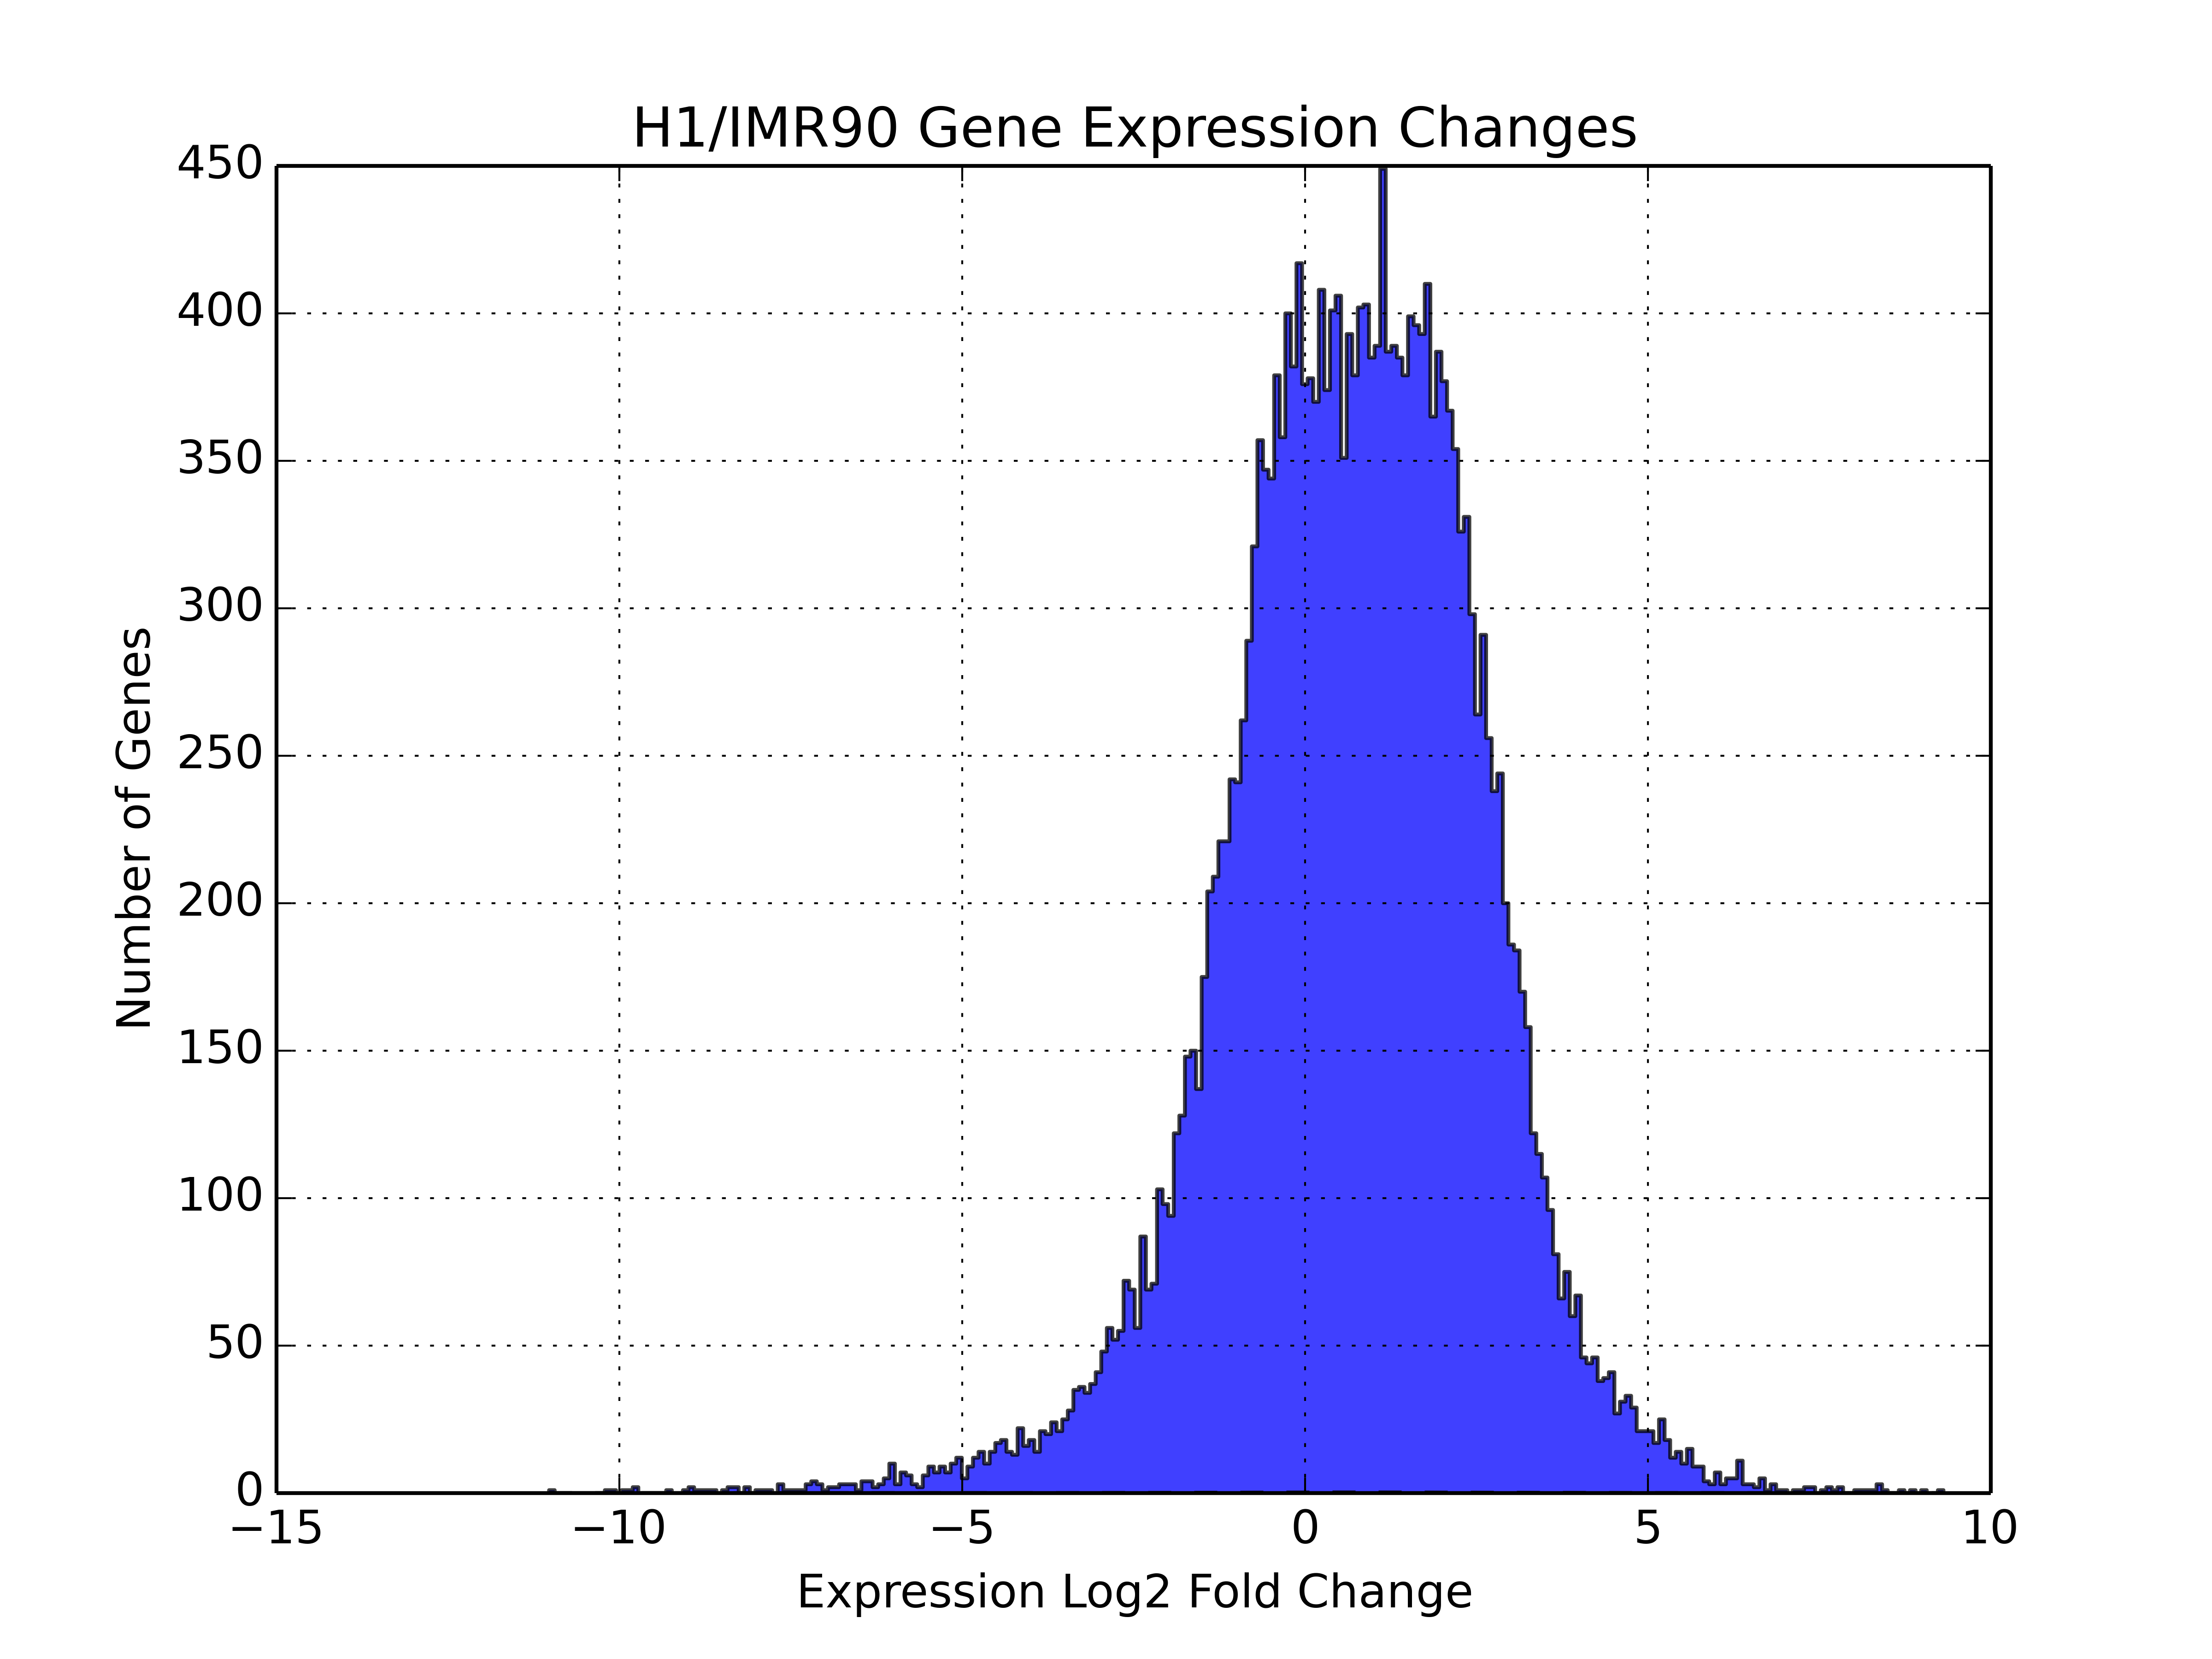
\includegraphics{./fig/supplementary/expressionDelta.png}\label{fig:subfigure3}
  }
  \caption{Gene Expression histograms for IMR90 and H1 hESCs.}\label{fig:gene-hist-supp}
\end{figure}


